\section{11.11.2014 - Porte logiche}

In questa esperienza verificheremo il funzionamento di alune porte logiche TTL e semplici circuiti costruiti con esse.

\subsection*{Strumenti e materiali}

%\begin{figure}[htc]
\begin{itemize} [noitemsep]
	%\item Generatore di forme d'onta Agilent 33120A con range di frequenza da \SI{100}{\micro\hertz} a \SI{15}{\mega\hertz};
	\item Oscilloscopio Agilent DSO-X 2002A (bandwidth \SI{70}{\mega\hertz}, sample rate \num{2} GSa/s);%\newline
%	\begin{minipage}{0.65\textwidth}
%		\vspace{0.4mm}
%%		\begin{itemize} [noitemsep]
%%		\item Oscilloscopio Agilent DSO-X 2002A (bandwidth \SI{70}{\mega\hertz}, sample rate \num{2} GSa/s);
		\item Generatore di tensione continua Agilent E3631A (max $\pm \, \SI{25}{\volt}$ o $\pm \, \SI{6}{\volt}$);
%%		\item Generatore di forme d'onta Agilent 33120A con range di frequenza da \SI{100}{\micro\hertz} a \SI{15}{\mega\hertz};
		\item Multimetro Agilent 34410A a sei cifre e mezza;
		\item Amplificatori operazionali OP07;
		\item Un integrato AD622 e un ISO124;
		\item Un integrato 7400;
		\item Basetta a LED;
		%\item Transistor di potenza NPN 2N2222;
		\item Porte logiche TTL;		
		\item Resistenze e capacità di vari valori;
		%\item Trimmer multigiro da \SI{10}{\kilo\ohm} e \SI{1}{\kilo\ohm};
		\item Breadboard e cablaggi vari.
%%		\end{itemize}
%	\end{minipage}
%	\begin{minipage}{0.3\textwidth}
%			\centering
%			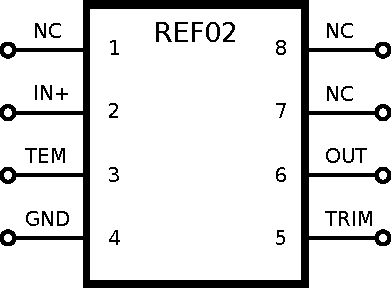
\includegraphics[width=3.5cm]{../E06/latex/REF02.pdf}
%			\caption{Piedinatura dell'integrato\newline REF02.}
%			\label{cir6:REF02}
%	\end{minipage}
\end{itemize}
%\end{figure}
%\vspace{-.8cm}


\subsection{Porte TTL e scheda di visualizzazione}
Le porte logiche a tecnologia TTL funzionano utilizzando come 1 logico il valore di tensione +\SI{5}{\volt} mentre come 0 logico \SI{0}{\volt}. Per controllare il funzionamento dei nostri circuiti utilizzeremo una schedina di visualizzazione a led. Tale circuito permette di visualizzare lo stato "alto" o "basso" delle linee da monitorare tramite 8 led (4 rossi e 4 verdi). Tali schede contengono un integrato buffer 74LS244 nella logica TTL che fornisce in uscita una corrente di \SI{-15}{\milli\ampere} per il livello alto e di \SI{24}{\milli\ampere} per il livello basso.
Ricordiamo che l'alimentazione deve essere stabilizzata e disaccoppiata con i condensatori come nel caso analogico in quanto nei momenti di commutazione delle porte abbiamo grandi variazioni di tensione in piccoli tempi (idealmente la variazione da stato 1 a 0 è istantanea). È dunque essenziale avere una riserva di cariche utilizzabili dal circuito nel momento in cui si hanno commutazioni.

\subsubsection{Porta NAND}


È stato montato il circuito come 


\begin{tabular}{|l|l|l|}
\hline
A & B & $\overline{AB}$ \\
\hline
0 & 0 & 1\\
\hline
0 & 1 & 1\\
\hline
1 & 0 & 1\\
\hline
1 & 1 & 0\\
\hline
\end{tabular}

\subsubsection{Porta NOT}


\begin{tabular}{|l|l|||l|l|}
\hline
$V_{in}$ [\si{\volt}] & $V_{out}$ [\si{\volt}] & $V_{in}$ [\si{\volt}]& $V_{out}$ [\si{\volt}]\\
\hline
0.5 &  & 3 &  \\
\hline
1 &  & 3.5 &  \\
\hline
1.5 &  & 4 &  \\
\hline
2 &  & 4.5 &  \\
\hline
2.5 &  & 5 &  \\
\hline
\end{tabular}


\subsubsection{Circuito di GATE}

\subsubsection{Porta XOR}

\subsubsection{Votazione con 3 Giurati e 1 Presidente}

\subsubsection{Allarme MINI-APPARTAMENTO}





